{\bf 2026-10-23}\\

Now that I have shown the jitter to be doing something that I would expect, let me try and apply it to a CMB map, instead of a point source map. I will use a 1 day scan of a simulated region similar to the Deep56 patch.


\begin{figure}
    \centering
    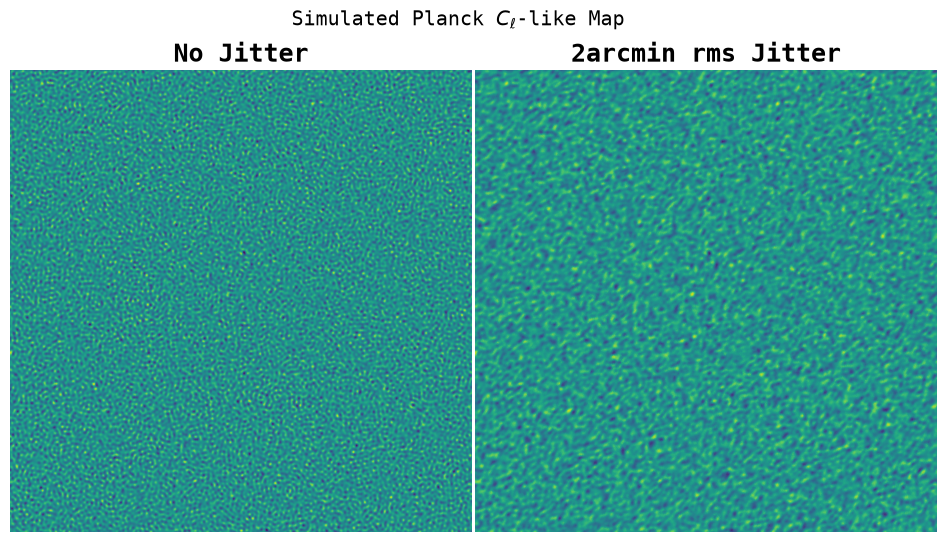
\includegraphics[width=0.75\textwidth]{Updates/figures/deep56_cmb_comp_map.png}
    \caption{Caption for the figure}
\end{figure}

\begin{figure}
    \centering
    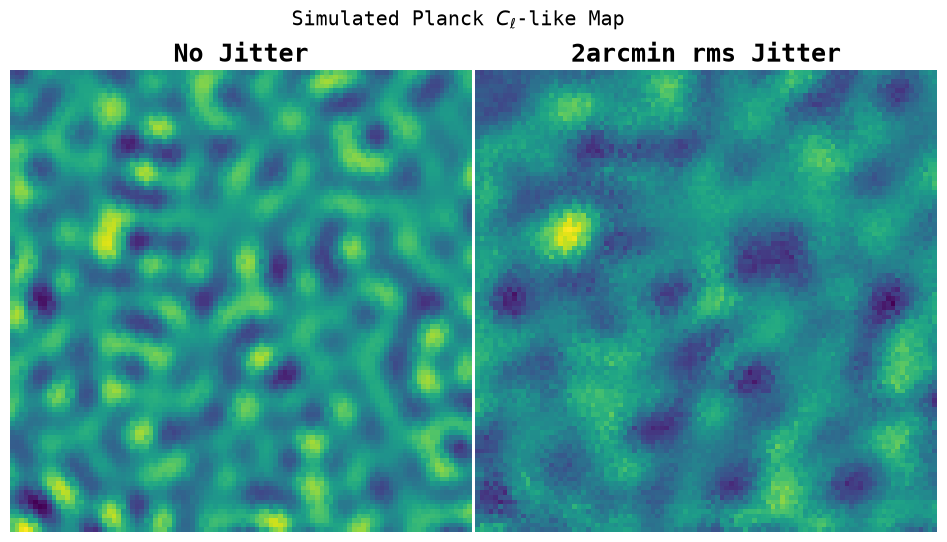
\includegraphics[width=0.75\textwidth]{Updates/figures/deep56_cmb_comp_map_zoom.png}
    \caption{Caption for the figure}
\end{figure}

I can look at what the the boresight pointing looks like compared to the nominal pointing. For 2 arcmin jitter ($\simeq 0.0333$ degrees), we would expect $\sim 68\%$ of the residuals to be within $\pm 0.0333$ degrees (assuming no sinusoidal component).

\begin{figure}
    \centering
    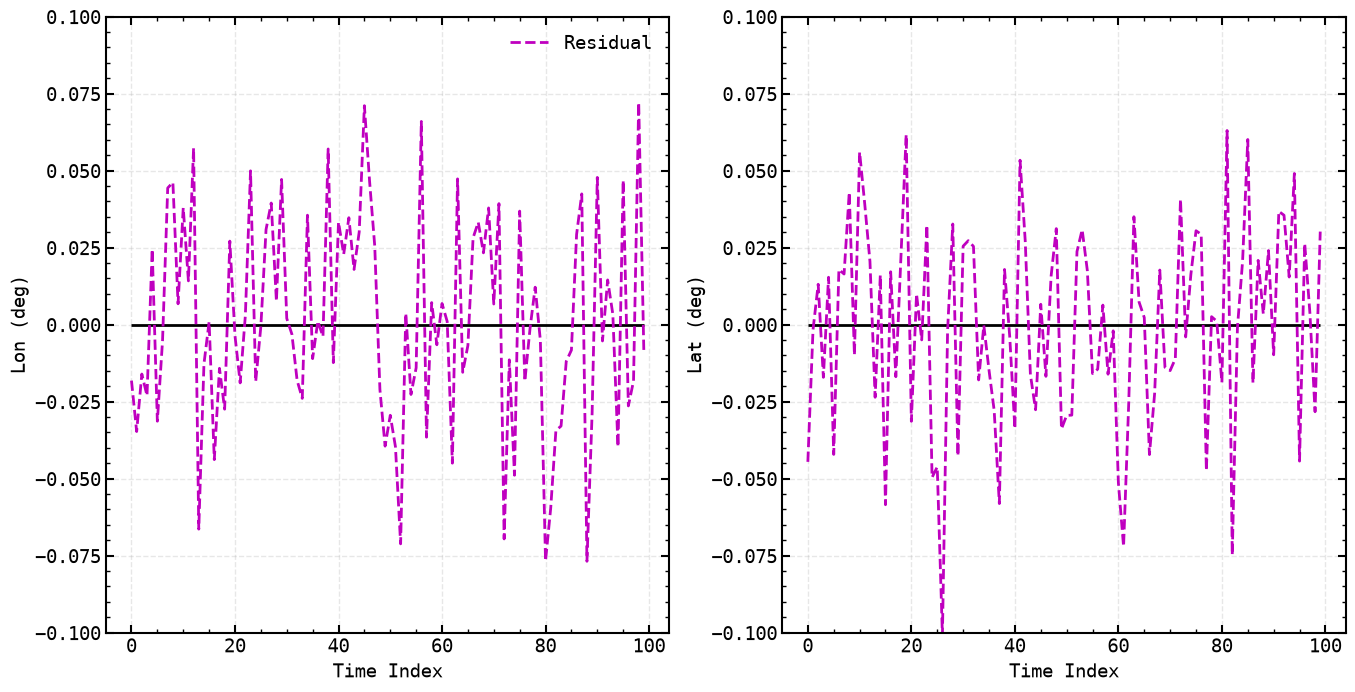
\includegraphics[width=0.75\textwidth]{Updates/figures/cmb_jitter_residual.png}
    \caption{Caption for the figure}
\end{figure}

How is the jitter actually defined:

First, we define a jitter standard deviation for each coordinate az $\sigma_{az}$, el $\sigma_{el}$, and $\psi$ $\sigma_{\psi}$ (in arcsec).

We draw an array from a Gaussian sample with length of the number of samples in the scan (or number of samples on the local data.obs) - I will call this $G_{az, el, \psi}$.

\pagebreak

\[
  S = A \sin{ft}
\]

\[
  \delta_{lon} = -\sigma_{az} \cdot \mathcal{Z}_{az} - A \sin{ft}
\]
\[
  \delta_{lat} = \sigma_{el} \cdot \mathcal{Z}_{el} + A \sin{ft}
\]
\[
  \delta_{\psi} = \sigma_{\psi} \cdot \mathcal{Z}_{\psi}
\]
